\section{Algoritmo Goloso}

\subsection{Soluci\'on}

Proponemos una solución heurística golosa para encontrar un conjunto dominante de un grafo lo mas pequeño posible con una complejidad polinomial.\\
Para ello nos basamos en una estrategia de selección de nodos dominantes, la cual consiste en elegir el nodo que mas adyacentes no cubiertas tenga (es decir, que todavía no fueron dominadas) y verificando en cada iteración si el conjunto actual es dominante. En base a diferentes estrategias y tipos de grafos (estrella, bipartitos, completos, estrellas unidas, caminos, ciclos) que fuimos observando, elegimos esta ya que fue la que más nos convenció y mejores resultados nos dió debido a que siempre intenta seleccionar el nodo que mas pueda dominar a otros nodos reduciendo el conjunto de los no cubiertos y acercándose a una mejor solución del problema. 

\subsection{Pseudocódigo}

\begin{codebox}
\Procname{$\proc{MCDGreedy}$ (\textbf{in} $Grafo$)}{conjuntoDomGoloso}{ConjDeVértices}
\li	vértices = lista de vértices del grafo	\RComment O(n)
\li	dominantes = conjunto vacio de vértices	
\li	\textbf{Mientras} no estén TodasCubiertas(vértices) \Do \RComment O($n^3$)
\li 		Ordeno los vértices por la cantidad adyacentes que tenga no cubiertas (sin dominar), de mayor a menor. \RComment O(n*log(n))
\li 		Elijo como dominante al primero de la lista y lo agrego al conjunto de \textbf{dominantes} \RComment O(n)
\li 		Saco de la lista de vértices al elegido \RComment O(n)
\li 		ActualizarGradoSinDominar(elegido) \RComment Actualizo los nodos del grafo,\\ disminuyendo la cantidad de \textit{grado sin dominar} de los adyacentes al elegido, y de los adyacentes a estos.  O($n^2$)
\End
\li	\textbf{return} dominantes
\end{codebox}

\begin{codebox}
\Procname{$\proc{TodasCubiertas}$ (\textbf{in} $ListaDeVertices$)}{result}{Boolean}
\li 	\textbf{Mientras} haya vértices en la lista \Do
\li 		\textbf{Si} el vértice no esta dominado \Do
\li 			\textbf{return} falso \End \End
\li 	\textbf{return} verdadero
\end{codebox}

\begin{codebox}
\Procname{$\proc{ActualizarGradoSinDominar}$ (\textbf{in} $Vertice$ $elegido$)}{}{}
\li 	Marcar al vértice elegido como dominado.
\li 	unionDeAdyacentes = lista de vértices vacía, que luego se usará para actualizar.
\li 	\textbf{Mientras} haya vértices en la lista de adyacentes al \textbf{elegido} \Do
\li 		\textbf{Si} el vértice \textit{elegido} no estaba dominado \Do
\li 			Decremento en uno el grado de adyacentes sin dominar del nodo actual \End
\li 		\textbf{Si} el nodo actual \textit{elegido} no estaba dominado \Do
\li 			Agrego los nodos adyacentes a la lista \textit{unionDeAdyacentes} \End
\li 		Marco al nodo actual como dominado. \End
\li 	\textbf{Mientras} haya vértices en la lista unionDeAdyacentes \Do 
\li 			Decremento en uno el grado de adyacentes sin dominar del nodo actual \End %\RComment Recorro unionDeAdyacentes para actualizar\\  el grado de nodos adyacentes sin dominar
\end{codebox}

\subsection{Análisis de Complejidad}

La complejidad del algoritmo es de O($n^3$)

El algoritmo comienza creando una lista de vértices en O(n).\\
Luego entra en un ciclo que como máximo será lineal en la cantidad de vértices. En cada iteración deberá comprobar si el conjunto actual de vértices elegidos domina todo el grafo en O($n^2$), ordenar todos los vértices en O(n*log(n)), elegir un vértice en O(1), removerlo de la lista en O(n) y finalmente actualizar el atributo de los grados sin dominar adyacentes de cada nodo en O($n^2$), esto es porque para los adyacentes del nodo elegido y a su vez para los adyacentes de estos tengo que bajar en uno este atributo, recorrer los adyacentes me lleva O(n) y por cada adyacente recorrer sus adyacentes también me lleva O(n), O(n) * O(n) = O($n^2$).\\

Por lo tanto, la complejidad nos queda:\\
O(n) + O(n) * (O($n^2$) + O(n*log(n) + O(n) + O($n^2$)) = O($n^3$)\\\\

La complejidad final del algoritmo goloso es de O($n^3$), cumpliendo el objetivo de ser polinomial.


\subsection{Peor Caso}

Al ser una heurística, en cierto casos la solución no es la óptima que podría dar un algoritmo exacto, pero aún asi es correcta.
Los peores casos, donde se produce una diferencia en el tamaño de conjunto dominante respecto a la optima, se suelen dar en grafos en los que varios nodos tienen el mismo grado o hay pequeña diferencia, y esto es debido que para la elección del vertice dominante en cada iteración nos quedamos con el que mayor grado de nodos adyacentes no cubiertos tenga y si hay varios con esta misma característica puede pasar que el nodo seleccionado no sea conveniente a futuro para llegar a una solución óptima.

En los siguientes ejemplos de grafos se puede apreciar mejor:

\begin {center}
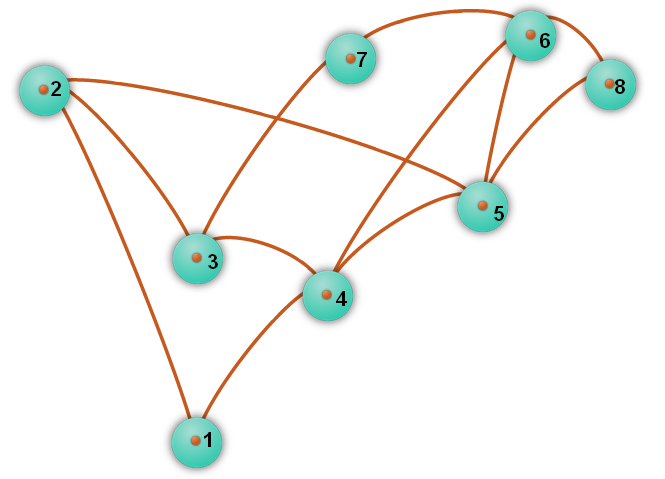
\includegraphics[width=8cm]{./graficos/grafo.png}
% grafico.eps: 0x0 pixel, 300dpi, 0.00x0.00 cm, bb=50 50 410 302
\end {center} 
La solución optima proporcionada por el algoritmo exacto es {6,2}, mientras que el goloso devuelve {4,3,5}, ya que como los nodos 6,4 y 5 tienen el mismo grado, al momento de la elección se decide por el 4 provocando esta diferencia en el tamaño del conjunto con respecto a la solución óptima.

\begin {center}
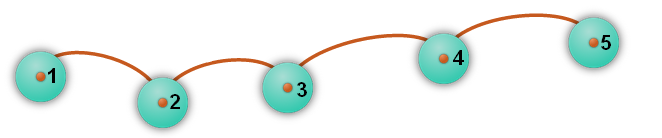
\includegraphics[width=8cm]{./graficos/grafo_camino.png}
% grafico.eps: 0x0 pixel, 300dpi, 0.00x0.00 cm, bb=50 50 410 302
\end {center} 
La solución óptima proporcionada por el algoritmo exacto es {2,4}, mientras que el goloso podría devolver {3,2,5}, ya que como los nodos 2, 3 y 4 tienen el mismo grado, si se decide por el 3, dejaría a todos los demás nodos con 1 grado sin dominar y faltando los dos extremos, provocando que si o si se necesite cubrirlos o elegirlos como dominantes, haciendo que el conjunto tenga tamaño 3 y no 2 como el exacto.

\subsection{Tests y análisis}

En los gráficos que aparece a continuación  se puede notar que a medida que la cantidad de nodos aumenta, el algoritmo dibuja un comportamiento que se asemeja a O($n^3$) en relación a la cantidad de ciclos y el tiempo en nanosegundos.\\

\begin {center}
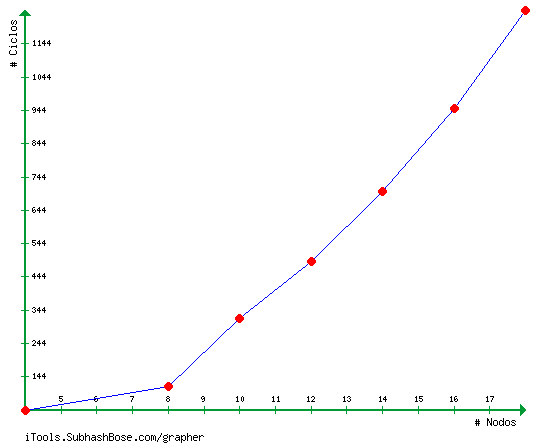
\includegraphics[width=8cm]{./graficos/goloso_1.png}
% grafico.eps: 0x0 pixel, 300dpi, 0.00x0.00 cm, bb=50 50 410 302
\end {center} 

\begin {center}
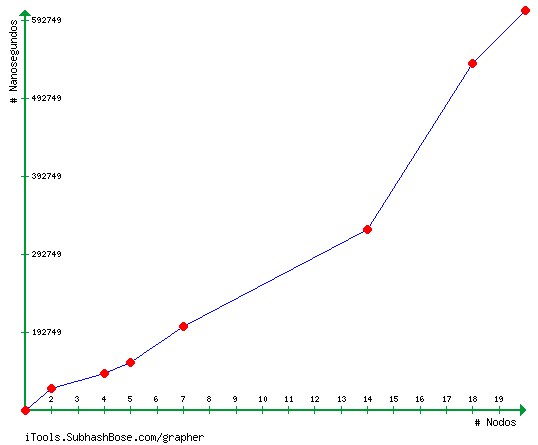
\includegraphics[width=8cm]{./graficos/goloso_2.png}
% grafico.eps: 0x0 pixel, 300dpi, 0.00x0.00 cm, bb=50 50 410 302
\end {center}
